% This is the University of Chicago Graham School Master of Science in Analytics
% template. Much of it is based on the Reed College LaTeX thesis template.
% Most of the work for the Reec College template was done by Sam Noble (SN),
% Later comments etc. by Ben Salzberg (BTS).
% Additional restructuring and APA support by Jess Youngberg (JY).
% Justin M. Shea (JMS) built on their good open source work.
% Your comments and suggestions are more than welcome:
% please email, them to justinshea@uchicago.edu.
%
% Any line that starts with a percent symbol is a comment.
% They won't show up in the document, and are useful for notes
% to yourself and explaining commands.
% Commenting also removes a line from the document;
% very handy for troubleshooting problems. -BTS
%%
%% Preamble
%%
% \documentclass{<something>} must begin each LaTeX document
% Added by JMS
\documentclass[12pt,oneside]{chicagocapstone}
% END of JMS add
% Packages are extensions to the basic LaTeX functions. Whatever you
% want to typeset, there is probably a package out there for it.
% Check out CTAN to see: http://www.ctan.org/
%%
\usepackage{graphicx,latexsym}
\usepackage{amsmath}
\usepackage{amssymb,amsthm}
\usepackage{longtable,booktabs,setspace}
\usepackage[hyphens]{url}
% Added by CII
\usepackage{hyperref}
\usepackage{lmodern}
\usepackage{float}
\floatplacement{figure}{H}
% End of CII addition
\usepackage{rotating}


% Added by CII (Thanks, Hadley!)
% Use ref for internal links
\renewcommand{\hyperref}[2][???]{\autoref{#1}}
\def\chapterautorefname{Chapter}
\def\sectionautorefname{Section}
\def\subsectionautorefname{Subsection}
% End of CII addition

% Added by CII
\usepackage{caption}
\captionsetup{width=5in}
% End of CII addition

% Added by JMS
\usepackage{mathptmx} % Times New Roman fonts
% End of add by JMS

% Syntax highlighting #22
  \usepackage{color}
  \usepackage{fancyvrb}
  \newcommand{\VerbBar}{|}
  \newcommand{\VERB}{\Verb[commandchars=\\\{\}]}
  \DefineVerbatimEnvironment{Highlighting}{Verbatim}{commandchars=\\\{\}}
  % Add ',fontsize=\small' for more characters per line
  \usepackage{framed}
  \definecolor{shadecolor}{RGB}{248,248,248}
  \newenvironment{Shaded}{\begin{snugshade}}{\end{snugshade}}
  \newcommand{\KeywordTok}[1]{\textcolor[rgb]{0.13,0.29,0.53}{\textbf{#1}}}
  \newcommand{\DataTypeTok}[1]{\textcolor[rgb]{0.13,0.29,0.53}{#1}}
  \newcommand{\DecValTok}[1]{\textcolor[rgb]{0.00,0.00,0.81}{#1}}
  \newcommand{\BaseNTok}[1]{\textcolor[rgb]{0.00,0.00,0.81}{#1}}
  \newcommand{\FloatTok}[1]{\textcolor[rgb]{0.00,0.00,0.81}{#1}}
  \newcommand{\ConstantTok}[1]{\textcolor[rgb]{0.00,0.00,0.00}{#1}}
  \newcommand{\CharTok}[1]{\textcolor[rgb]{0.31,0.60,0.02}{#1}}
  \newcommand{\SpecialCharTok}[1]{\textcolor[rgb]{0.00,0.00,0.00}{#1}}
  \newcommand{\StringTok}[1]{\textcolor[rgb]{0.31,0.60,0.02}{#1}}
  \newcommand{\VerbatimStringTok}[1]{\textcolor[rgb]{0.31,0.60,0.02}{#1}}
  \newcommand{\SpecialStringTok}[1]{\textcolor[rgb]{0.31,0.60,0.02}{#1}}
  \newcommand{\ImportTok}[1]{#1}
  \newcommand{\CommentTok}[1]{\textcolor[rgb]{0.56,0.35,0.01}{\textit{#1}}}
  \newcommand{\DocumentationTok}[1]{\textcolor[rgb]{0.56,0.35,0.01}{\textbf{\textit{#1}}}}
  \newcommand{\AnnotationTok}[1]{\textcolor[rgb]{0.56,0.35,0.01}{\textbf{\textit{#1}}}}
  \newcommand{\CommentVarTok}[1]{\textcolor[rgb]{0.56,0.35,0.01}{\textbf{\textit{#1}}}}
  \newcommand{\OtherTok}[1]{\textcolor[rgb]{0.56,0.35,0.01}{#1}}
  \newcommand{\FunctionTok}[1]{\textcolor[rgb]{0.00,0.00,0.00}{#1}}
  \newcommand{\VariableTok}[1]{\textcolor[rgb]{0.00,0.00,0.00}{#1}}
  \newcommand{\ControlFlowTok}[1]{\textcolor[rgb]{0.13,0.29,0.53}{\textbf{#1}}}
  \newcommand{\OperatorTok}[1]{\textcolor[rgb]{0.81,0.36,0.00}{\textbf{#1}}}
  \newcommand{\BuiltInTok}[1]{#1}
  \newcommand{\ExtensionTok}[1]{#1}
  \newcommand{\PreprocessorTok}[1]{\textcolor[rgb]{0.56,0.35,0.01}{\textit{#1}}}
  \newcommand{\AttributeTok}[1]{\textcolor[rgb]{0.77,0.63,0.00}{#1}}
  \newcommand{\RegionMarkerTok}[1]{#1}
  \newcommand{\InformationTok}[1]{\textcolor[rgb]{0.56,0.35,0.01}{\textbf{\textit{#1}}}}
  \newcommand{\WarningTok}[1]{\textcolor[rgb]{0.56,0.35,0.01}{\textbf{\textit{#1}}}}
  \newcommand{\AlertTok}[1]{\textcolor[rgb]{0.94,0.16,0.16}{#1}}
  \newcommand{\ErrorTok}[1]{\textcolor[rgb]{0.64,0.00,0.00}{\textbf{#1}}}
  \newcommand{\NormalTok}[1]{#1}

% To pass between YAML and LaTeX the dollar signs are added by CII
\title{Forecasting Coca-Cola Bag Orders Using Social Media}
\author{Elijah Ampo, Ruohan Zhou, and Yingkun Zhu}
\date{May, 2019} % The month and year that you submit your FINAL draft)
\division{Graham School}
\advisor{Arnab Bose}
\institution{University of Chicago}
\degree{Master of Science in Analytics}
\altadvisor{Dr.~Sema Barlas}
% End of CII addition

\department{Continuing Liberal and Professional Studies}

% Added by CII
%%% Copied from knitr
%% maxwidth is the original width if it's less than linewidth
%% otherwise use linewidth (to make sure the graphics do not exceed the margin)
\makeatletter
\def\maxwidth{ %
  \ifdim\Gin@nat@width>\linewidth
    \linewidth
  \else
    \Gin@nat@width
  \fi
}
\makeatother

\renewcommand{\contentsname}{Table of Contents}
% End of CII addition

\setlength{\parskip}{0pt}

% Added by CII
  %\setlength{\parskip}{\baselineskip}
  \usepackage[parfill]{parskip}

\providecommand{\tightlist}{%
  \setlength{\itemsep}{0pt}\setlength{\parskip}{0pt}}


\Abstract{
Scholle IPN is a global manufacturing company that has experienced
variability in their sales forecasts. In this project, we will
demonstrate how Scholle IPN can leverage social media data to predict
orders from their clients. We will introduce dimension reduction methods
to account for the high dimensional nature of social media data. In
addition, an ensemble model approach to sales forecasting will be used
to generate the best sales forecasting model.

\bigskip  \bigskip
\bigskip

\textbf{Keywords}: Time Series, Machine Learning, sARIMA, Regression
with ARIMA Errors, XGBoost, Long Short-Term Memory (LSTM), Ensemble,
Social Media, Linear Regression.

\bigskip  \bigskip
\bigskip
}

% Added by JMS
\Executive{
Manufacturing companies need to forecast the demand of their products
ahead of time, so that raw material preparation, production, and
shipping schedule can be arranged accordingly. Failing to predict the
future demand can result in waste due to over-producing, business
opportunities lose because of under-stocking or unable to deliver in a
timely manner, etc. In an era where social media dominates people's
life, and data analytics are growing more and more powerful when it
comes to drawing insights to enhance business actions, Scholle IPN
tasked us to test if Social Media brings any predictive power to
forecast the future Coca-Cola bag sales. With this problem stated, we
took this task on as a trial to examine whether or not people's
discussion and engagement on Social Media has any impact on the
consumption of the Coke product in real life.

In order to achieve that, we started with gathering external data from
Social Media, and combined with the internal data provided by Scholle
IPN. After preliminary exploratory on the data - both internal and
external, we built traditional Regression with ARIMA errors models, then
more advanced Machine Learning models, namely, XGBoost and LSTM RNN.
XGBoost using the differenced social media variables gave the best
predictions (lowest sMAPE score) among all the individual models while
still has a decent level of interpretability for us to explain the
model. Since we obtained the various predicting results from the single
predicting models, we also stacked these individual models together and
created three ensemble models - mean average, Linear Regression, and
Random Forest. Random Forest ensemble model achieved the best outcomes,
with the lowest error score. Key findings from this project including
the following:
\begin{itemize}
\tightlist
\item
  Social Media contents, specifically, online discussions and engagement
  level of certain brands and ad campaigns have helped Machine Learning
  models to forecast the future bag sales.
\item
  Different Social Media variables have different importances when it
  comes to modeling. For instance, the jobs related conversation online
  demonstrated higher level of importance than other brands-related
  conversations in our XGBoost model feature importance.
\item
  Reducing the dimensionality when handling a large number of features
  improves the predictive accuracy; Cross Correlation check, Principal
  Component Analysis are also vital before modeling in our case.
\item
  Ensemble modeling is a great way to bring the individual models
  together as inputs, and establish a better model with stronger
  predictive capacity. The output from the ensemble model has been
  proven to be the best results out of all. We recommend Scholle IPN to
  continue monitoring the Social Media conversations, and follow our
  practice of adding the social media variables to the internal
  historical sales data. For future work, we also recommend to examine
  the year-to-year comparison between the forecasting bag sales with the
  actual bag sales.
\end{itemize}
}
% End of JMS add

\Acknowledgements{

}

\Dedication{

}

\Preface{

}


% End of CII addition
%%
%% End Preamble
%%
%
\begin{document}

% Everything below added by CII
  \maketitle

\frontmatter % this stuff will be roman-numbered
\pagestyle{empty} % this removes page numbers from the frontmatter


%% Reorganized by JMS
  \begin{abstract}
    Scholle IPN is a global manufacturing company that has experienced
    variability in their sales forecasts. In this project, we will
    demonstrate how Scholle IPN can leverage social media data to predict
    orders from their clients. We will introduce dimension reduction methods
    to account for the high dimensional nature of social media data. In
    addition, an ensemble model approach to sales forecasting will be used
    to generate the best sales forecasting model.
    
    \bigskip  \bigskip
    \bigskip
    
    \textbf{Keywords}: Time Series, Machine Learning, sARIMA, Regression
    with ARIMA Errors, XGBoost, Long Short-Term Memory (LSTM), Ensemble,
    Social Media, Linear Regression.
    
    \bigskip  \bigskip
    \bigskip
  \end{abstract}
 % Added by JMS
  \begin{executive}
    Manufacturing companies need to forecast the demand of their products
    ahead of time, so that raw material preparation, production, and
    shipping schedule can be arranged accordingly. Failing to predict the
    future demand can result in waste due to over-producing, business
    opportunities lose because of under-stocking or unable to deliver in a
    timely manner, etc. In an era where social media dominates people's
    life, and data analytics are growing more and more powerful when it
    comes to drawing insights to enhance business actions, Scholle IPN
    tasked us to test if Social Media brings any predictive power to
    forecast the future Coca-Cola bag sales. With this problem stated, we
    took this task on as a trial to examine whether or not people's
    discussion and engagement on Social Media has any impact on the
    consumption of the Coke product in real life.
    
    In order to achieve that, we started with gathering external data from
    Social Media, and combined with the internal data provided by Scholle
    IPN. After preliminary exploratory on the data - both internal and
    external, we built traditional Regression with ARIMA errors models, then
    more advanced Machine Learning models, namely, XGBoost and LSTM RNN.
    XGBoost using the differenced social media variables gave the best
    predictions (lowest sMAPE score) among all the individual models while
    still has a decent level of interpretability for us to explain the
    model. Since we obtained the various predicting results from the single
    predicting models, we also stacked these individual models together and
    created three ensemble models - mean average, Linear Regression, and
    Random Forest. Random Forest ensemble model achieved the best outcomes,
    with the lowest error score. Key findings from this project including
    the following:
    \begin{itemize}
    \tightlist
    \item
      Social Media contents, specifically, online discussions and engagement
      level of certain brands and ad campaigns have helped Machine Learning
      models to forecast the future bag sales.
    \item
      Different Social Media variables have different importances when it
      comes to modeling. For instance, the jobs related conversation online
      demonstrated higher level of importance than other brands-related
      conversations in our XGBoost model feature importance.
    \item
      Reducing the dimensionality when handling a large number of features
      improves the predictive accuracy; Cross Correlation check, Principal
      Component Analysis are also vital before modeling in our case.
    \item
      Ensemble modeling is a great way to bring the individual models
      together as inputs, and establish a better model with stronger
      predictive capacity. The output from the ensemble model has been
      proven to be the best results out of all. We recommend Scholle IPN to
      continue monitoring the Social Media conversations, and follow our
      practice of adding the social media variables to the internal
      historical sales data. For future work, we also recommend to examine
      the year-to-year comparison between the forecasting bag sales with the
      actual bag sales.
    \end{itemize}
  \end{executive}
 % End of JMS




  \hypersetup{linkcolor=black}
  \setcounter{tocdepth}{2}
  \tableofcontents

  \listoffigures

  \listoftables

%% END of Reorganization by JMS

\mainmatter % here the regular arabic numbering starts
\pagestyle{fancyplain} % turns page numbering back on

\chapter*{Introduction}\label{introduction}
\addcontentsline{toc}{chapter}{Introduction}

Scholle IPN is a global manufacturing company based in Northlake, IL,
with products focused primarily in bag-in-box packaging. The company is
a pioneer in its industry by implementing a combination of qualitative
observations and quantitative analyses in forecasting their products'
sales. However, variability in these sales forecasts present challenges
for Scholle IPN in raw material preparation, operational efficiency, and
asset management.

\section*{Problem Statement}\label{problem-statement}
\addcontentsline{toc}{section}{Problem Statement}

In this project, we will provide a forecasting solution to Scholle IPN
using social media data. This project will primarily focus on one of
Scholle IPN's main clients, Coca-Cola. Coca-Cola uses Scholle IPN's
state-of-the art bags to store beverage products at quick service
restaurant (QSR) partners worldwide. Since 2014, Coca-Cola has accounted
for 95.68\% of Scholle's syrup-related bag order shipments, so
inaccurate forecasts of future orders could result in operational
inefficiencies. Minimizing these operational inefficiencies is important
to maintain Scholle's partnership with Coca-Cola. In order to solve this
business problem, we will examine whether we can substantially improve
Scholle IPN's Coca-Cola demand forecasts by using social media as the
primary variable.

\section*{Research Purpose}\label{research-purpose}
\addcontentsline{toc}{section}{Research Purpose}

The purpose of this research is to forecast Coca-Cola bag orders by
utilizing social media data. When customer express their opinions in
social media, businesses like Scholle IPN can gain valuable insights
that can inform business decisions. For example, if a McDonald's
promotion is generating discussion posts online, then Scholle IPN can
potentially expect an increase in bag orders from Coca-Cola. In order to
make these online discussions actionable, we must first take into
account additional considerations. First, since social media posts are
usually in the form of text, we will explore methods to convert text to
numerical data. Second, we will need to explore different ways to reduce
the dimension of social media variables to account for its high
dimensionality. And finally, we will use these social media variables to
forecast Coca-Cola bag orders using an ensemble approach. Below is a
list of research objectives for this project:
\begin{itemize}
\tightlist
\item
  Convert text-based social media data to numerical data using natural
  language processing.
\item
  Reduce the dimension of social media variables using different
  methods.
\item
  Forecast Coca-Cola bag orders using an ensemble approach.
\end{itemize}
\section*{Variables and Scope}\label{variables-and-scope}
\addcontentsline{toc}{section}{Variables and Scope}

The scope of this forecasting project will be limited to predicting the
future monthly bag orders for Coca-Cola in the United States and Canada.
All variables will be aggregated or averaged at the monthly level. The
forecasting window for this project will be 18 months for all models to
accommodate Scholle's business needs. The main social media variables
used to predict Coca-Cola bag orders will be collected from Twitter and
Google Trends. For Twitter, we will focus our project on the following
variables: tweet text, number of likes, number of retweets, and number
of replies. For Google Trends, monthly trend values for selected topics
will be extracted at the monthly level. Additional data retrieval rules
were applied to ensure that Twitter and Google Trends data are from the
United States and Canada (see Appendix A).

\chapter*{Background}\label{background}
\addcontentsline{toc}{chapter}{Background}

1.Social Media Variables For this forecasting project, we will focus on
collecting social media data on relevant topics. These relevant topics
are Coca-Cola, Pepsi, McDonald's, Taco Bell, and ``jobs''. Coca-Cola was
selected because it is their product's demand that Scholle IPN is
interested in forecasting. Pepsi was selected due to its position as the
main competitor for Coca-Cola. Meanwhile, McDonald's and Taco Bell were
chosen because they are the top quick service restaurant partners for
Coca-Cola and Pepsi based on 2018 annual sales revenue. The topic `jobs'
was selected to gather job-related tweets intended to capture economic
activity in the United States and Canada. Relationships between social
media activity on these topics and the quantity of Coca-Cola bag ordered
can be useful information for our forecasting models. Twitter data will
be a combination of user-level tweets and company-level tweets, while
Google Trend data will be a monthly trend value for our selected terms.
User-level tweets are Twitter posts from regular online consumers
tweeting about Coca-Cola, Pepsi, McDonald's, Taco Bell, and ``jobs.''
Company-level tweets are Twitter posts by the official Twitter accounts
of Coca-Cola, Pepsi, McDonald's, and Taco Bell. Meanwhile, Google Trends
is a popularity measure for Coca-Cola and other relevant terms based on
their search frequency over time.

2.Sentiment Analysis One method of quantifying text-based social media
data for our forecasting models is by implementing sentiment analysis.
This is a technique in natural language processing that we will use for
each tweet to generate a numerical value signifying whether consumers
have a positive or negative outlook on Coca-Cola, Pepsi, McDonald's,
Taco Bell, or jobs. We can then average sentiment scores by month for
each relevant term, and use this as an additional predictor to forecast
Coca-Cola bag orders. For this project, we will only calculate sentiment
scores for user-generated tweets because we assume that tweets generated
by the official company accounts are all positive. Prior to conducting
sentiment analysis, text processing steps must be conducted on tweets.
The following steps were conducted on the tweets: \emph{Remove stop
words on tweets }Tokenize tweets *Lemmatize tweets\\
The R package sentimentR was used to calculate sentiment scores for each
tweet. This package takes into account additional information such as
valence shifters and de-amplifiers resulting in a more accurate
sentiment score (see Appendix A). The sentiment scores for each selected
term's collective tweets per month will be averaged at the monthly level
to generate the monthly average sentiment variable.

3.Stationarity and Defferencing An important step to consider when
forecasting is to remove trends and seasonality from variables in order
to make it stationary. When time series data is stationary displaying a
stable mean and stable variance over time, it is less likely to produce
spurious relationships and misleading results. Statistical tests (KPSS
test) were conducted on each variable to determine its stationarity (see
Appendix A). After testing, it was determined that the dependent
variable, monthly quantity of Coca-Cola bag orders, was stationary. This
means that this variable requires no further transformations. However,
the independent variables showed varying results and require additional
processing. One way of transforming time series data to become
stationary is the method of differencing. Differencing is the method of
subtracting the value of the current time step from the value of
previous time step(s). This method was applied to all social media
variables to ensure that they were all stationary. The visual below
demonstrates how the method of differencing is able to remove trends
from the monthly total user tweets. The top half of the visual are time
plots of the pre-differenced variables, while the bottom are time plots
of the differenced variables.
\begin{Shaded}
\begin{Highlighting}[]
\KeywordTok{include_graphics}\NormalTok{(}\DataTypeTok{path =} \StringTok{"figure/differencing.jpg"}\NormalTok{)}
\end{Highlighting}
\end{Shaded}
\begin{figure}

{\centering 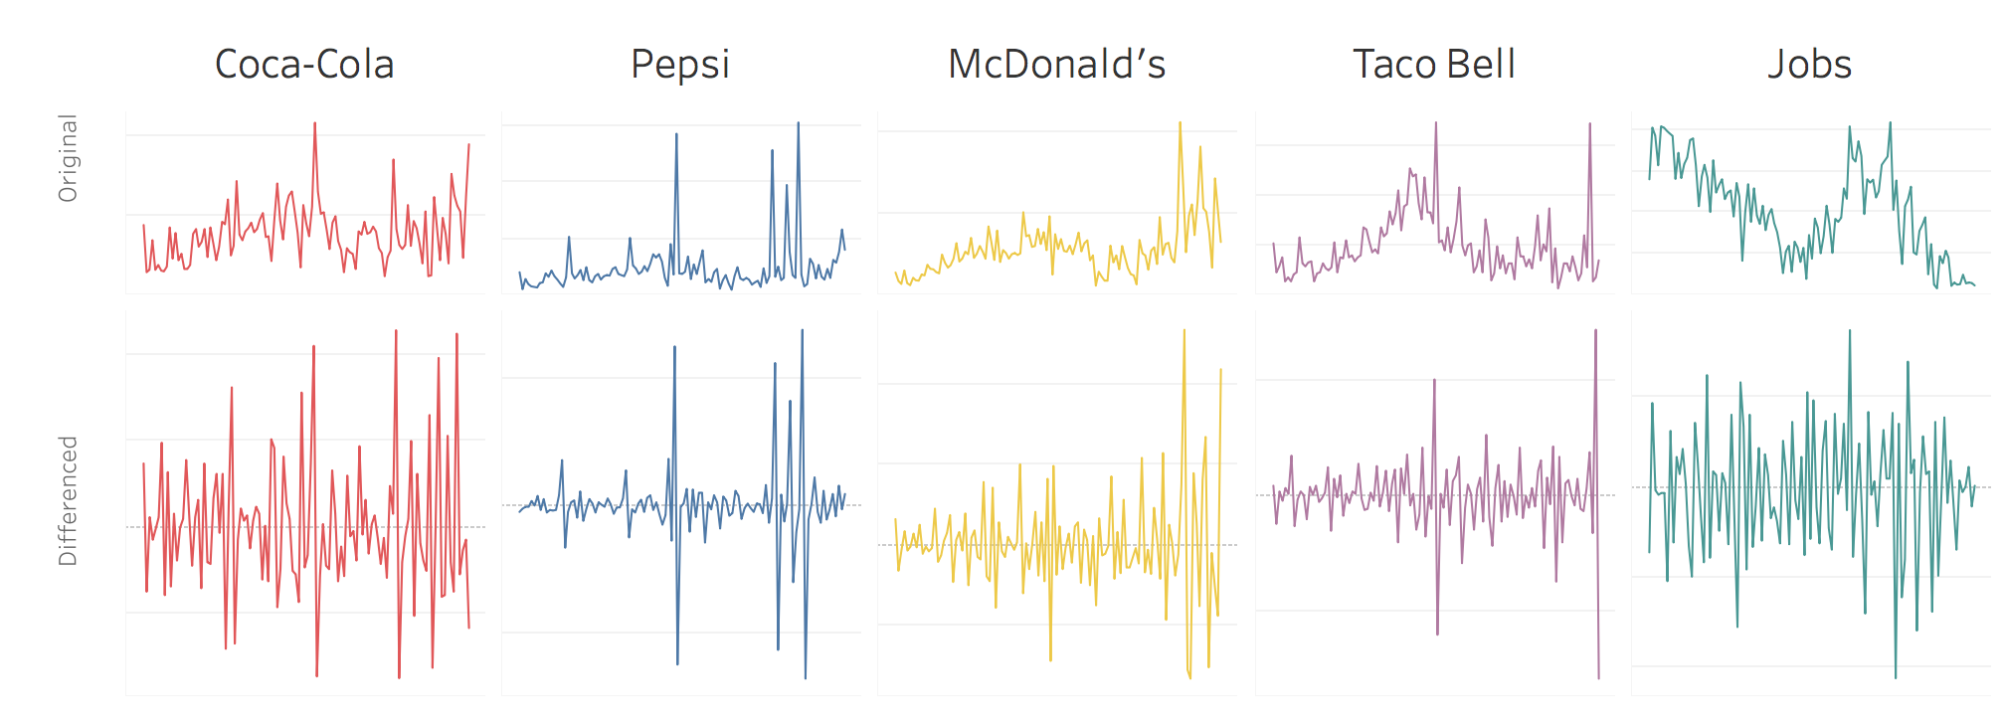
\includegraphics[width=200px]{figure/differencing} 

}

\caption{differenced social media data}\label{fig:differencing}
\end{figure}
4.Dimension Reduction When building forecasting models, it is important
to be aware of the level of complexity of these models. In this project,
we will be collecting Twitter data that allow users to collect over a
hundred features for a single tweet (tweet text, user profile data,
etc.). Using all of these variables will make our forecasting models
highly complex and likely result in poor predictions. Fortunately, the
scope of this project limits tweet information to only a tweet's text,
number of likes, number of retweets, and number of replies. However, the
complexity of this project (relevant topics, social media data type,
social media source) still leaves us with 46 total independent variables
per observation (see Data section). We will use two main approaches in
this project to further reduce our social media variable's dimensions.

*Method A - Principal Component Analysis\\
The first method we will use to reduce the dimensionality of our social
media variables is principal component analysis (PCA). PCA uses an
orthogonal transformation of our variables into linearly uncorrelated
variables called principal components. The main idea is that the
majority of the variance explained will be concentrated on a limited
number of principal components. This allows us to discard the principal
component variables that provide little additional information. This
approach further reduces the overall dimension of our original set of
variables. When performing this technique with our social media
variables, we are able to observe the ``elbow feature'' at number of
principal component (n) = 7 . This tells us that only the first seven
principal components is required to explain most of the total variance
(97\%) of our variables. By using PCA, we were able to reduce our
overall social media variables from 46 to 7.
\begin{Shaded}
\begin{Highlighting}[]
\KeywordTok{include_graphics}\NormalTok{(}\DataTypeTok{path =} \StringTok{"figure/pca.jpg"}\NormalTok{)}
\end{Highlighting}
\end{Shaded}
\begin{figure}

{\centering 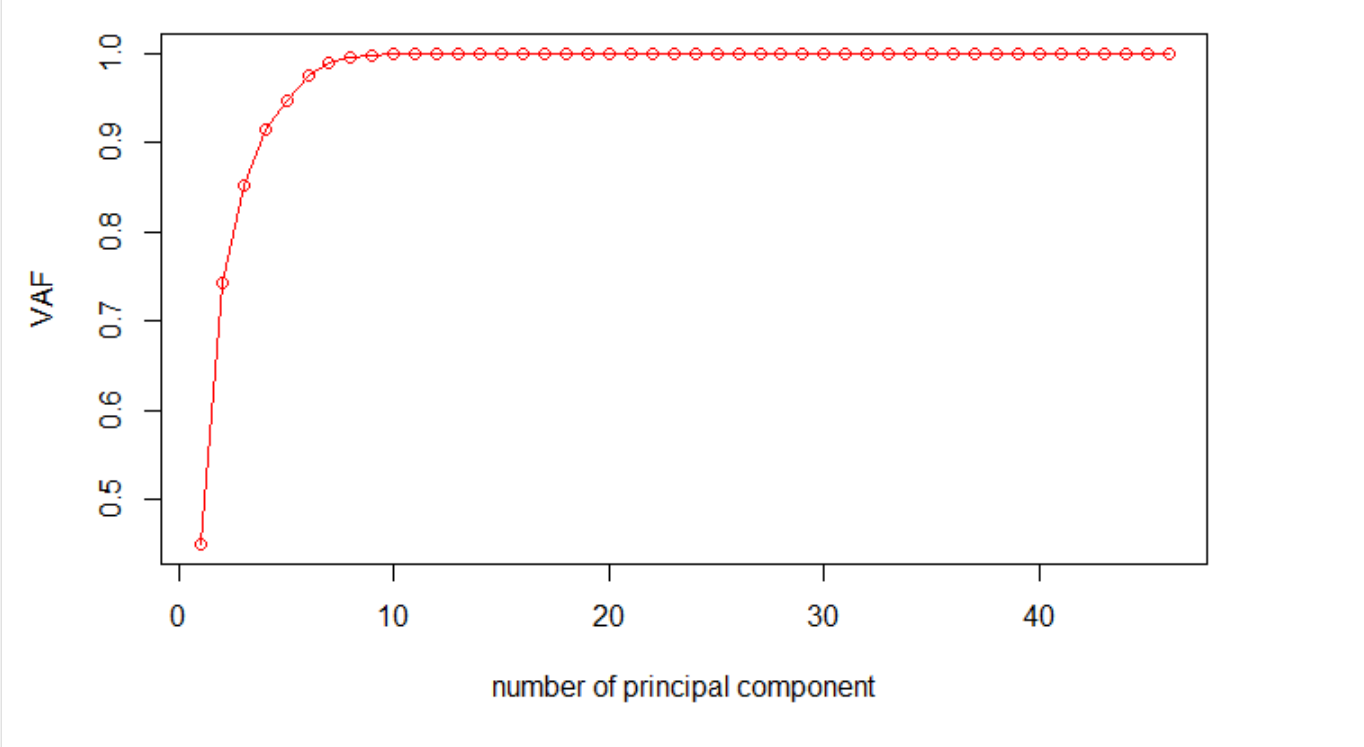
\includegraphics[width=200px]{figure/pca} 

}

\caption{Principal Component Analysis}\label{fig:pca}
\end{figure}
*Method B - Cross Correlation The second method we will employ to reduce
our total features is by testing our independent variables for cross
correlation with the dependent variable. Mainly, this approach will
inform us on how many months in advance a social media variable can lead
to an increase or decrease in Coca-Cola bag orders. For example,
consider when a social media variable was found to be significantly
positively correlated with Coca-Cola bag orders at lag t-1. If this
social media variable has a positive value for the current month, then
an increase in Coca-Cola bag orders can be expected the following month.
In this project, we will check for cross correlation on each independent
variable up to six months prior (t-6). We will do this on the original
variables as well as the principal component variables. Using the cross
correlation approach, we were able to identify eight lags from the
social media variables that were cross correlated with Coca-Cola bag
orders. Below is a table of these social media variables with their
specified lags listed.
\begin{longtable}[]{@{}cc@{}}
\caption{\label{tab:inher} Social Media Variables with Specified
Lags}\tabularnewline
\toprule
\begin{minipage}[b]{0.34\columnwidth}\centering\strut
Social Media Variable\strut
\end{minipage} & \begin{minipage}[b]{0.43\columnwidth}\centering\strut
Significant Lag\strut
\end{minipage}\tabularnewline
\midrule
\endfirsthead
\toprule
\begin{minipage}[b]{0.34\columnwidth}\centering\strut
Social Media Variable\strut
\end{minipage} & \begin{minipage}[b]{0.43\columnwidth}\centering\strut
Significant Lag\strut
\end{minipage}\tabularnewline
\midrule
\endhead
\begin{minipage}[t]{0.34\columnwidth}\centering\strut
Coca-Cola Account tweet\strut
\end{minipage} & \begin{minipage}[t]{0.43\columnwidth}\centering\strut
s t-1\strut
\end{minipage}\tabularnewline
\begin{minipage}[t]{0.34\columnwidth}\centering\strut
Taco Bell Account tweet\strut
\end{minipage} & \begin{minipage}[t]{0.43\columnwidth}\centering\strut
s t-1\strut
\end{minipage}\tabularnewline
\begin{minipage}[t]{0.34\columnwidth}\centering\strut
Job Google Trend\strut
\end{minipage} & \begin{minipage}[t]{0.43\columnwidth}\centering\strut
t-2\strut
\end{minipage}\tabularnewline
\begin{minipage}[t]{0.34\columnwidth}\centering\strut
McDonald's Google Trend\strut
\end{minipage} & \begin{minipage}[t]{0.43\columnwidth}\centering\strut
t-2\strut
\end{minipage}\tabularnewline
\begin{minipage}[t]{0.34\columnwidth}\centering\strut
McDonald's Account repli\strut
\end{minipage} & \begin{minipage}[t]{0.43\columnwidth}\centering\strut
es t-5\strut
\end{minipage}\tabularnewline
\begin{minipage}[t]{0.34\columnwidth}\centering\strut
Taco Bell Google Trend\strut
\end{minipage} & \begin{minipage}[t]{0.43\columnwidth}\centering\strut
t-5\strut
\end{minipage}\tabularnewline
\begin{minipage}[t]{0.34\columnwidth}\centering\strut
McDonald's Google Trend\strut
\end{minipage} & \begin{minipage}[t]{0.43\columnwidth}\centering\strut
t-5\strut
\end{minipage}\tabularnewline
\begin{minipage}[t]{0.34\columnwidth}\centering\strut
Pepsi Account tweets\strut
\end{minipage} & \begin{minipage}[t]{0.43\columnwidth}\centering\strut
t-6\strut
\end{minipage}\tabularnewline
\bottomrule
\end{longtable}
In addition, we were able to identify seven lags from principal
components that were cross correlated with Coca-Cola bag orders. Below
is a table of these principal components with their specified lags
listed.
\begin{longtable}[]{@{}cc@{}}
\caption{\label{tab:inher} Principal Components with Specified
Lags}\tabularnewline
\toprule
\begin{minipage}[b]{0.34\columnwidth}\centering\strut
Principal Component\strut
\end{minipage} & \begin{minipage}[b]{0.43\columnwidth}\centering\strut
Significant Lag\strut
\end{minipage}\tabularnewline
\midrule
\endfirsthead
\toprule
\begin{minipage}[b]{0.34\columnwidth}\centering\strut
Principal Component\strut
\end{minipage} & \begin{minipage}[b]{0.43\columnwidth}\centering\strut
Significant Lag\strut
\end{minipage}\tabularnewline
\midrule
\endhead
\begin{minipage}[t]{0.34\columnwidth}\centering\strut
PC7\strut
\end{minipage} & \begin{minipage}[t]{0.43\columnwidth}\centering\strut
t-1\strut
\end{minipage}\tabularnewline
\begin{minipage}[t]{0.34\columnwidth}\centering\strut
PC6\strut
\end{minipage} & \begin{minipage}[t]{0.43\columnwidth}\centering\strut
t-2\strut
\end{minipage}\tabularnewline
\begin{minipage}[t]{0.34\columnwidth}\centering\strut
PC4\strut
\end{minipage} & \begin{minipage}[t]{0.43\columnwidth}\centering\strut
t-2\strut
\end{minipage}\tabularnewline
\begin{minipage}[t]{0.34\columnwidth}\centering\strut
PC6\strut
\end{minipage} & \begin{minipage}[t]{0.43\columnwidth}\centering\strut
t-3\strut
\end{minipage}\tabularnewline
\begin{minipage}[t]{0.34\columnwidth}\centering\strut
PC4\strut
\end{minipage} & \begin{minipage}[t]{0.43\columnwidth}\centering\strut
t-3\strut
\end{minipage}\tabularnewline
\begin{minipage}[t]{0.34\columnwidth}\centering\strut
PC3\strut
\end{minipage} & \begin{minipage}[t]{0.43\columnwidth}\centering\strut
t-5\strut
\end{minipage}\tabularnewline
\begin{minipage}[t]{0.34\columnwidth}\centering\strut
PC3\strut
\end{minipage} & \begin{minipage}[t]{0.43\columnwidth}\centering\strut
t-6\strut
\end{minipage}\tabularnewline
\bottomrule
\end{longtable}
5.Ensemble Modeling A variety of different machine learning models will
be used to forecast future Coca-Cola bag orders (see Modeling
Framework). In addition to these machine learning models, this project
will demonstrate the strength of the ensemble model approach. The main
assumption to ensemble modeling is that combining all lower-level models
will result in a more accurate, overall model. An ensemble model is able
to highlight the strength of each individual model and account for each
model's weaknesses. The ensemble model approach will be used in this
project to produce the best model.

\newpage

\chapter*{Methodology}\label{methodology}
\addcontentsline{toc}{chapter}{Methodology}

\section*{Data}\label{methodology-data}
\addcontentsline{toc}{section}{Data}

The data used to predict Coca-Cola bag orders will come from three
distinct sources: Scholle IPN, Twitter, and Google Trends. The
aggregation of all relevant data will be at the monthly level with a
date range from October 2009 to October 2018. This will ensure that the
data will have enough observations for our forecasting models. The
dependent variable for this project will be the monthly total bag orders
from Coca-Cola, which will be calculated using Scholle IPN's internal
sales data. The independent variables are social media variables
collected from Twitter and Google Trends. Twitter is a widely used
social media platform in the United States and Canada that was founded
in 2006. This platform will allow us to get a feeling about users and
their opinions on Coca-Cola, Pepsi, McDonald's, Taco Bell, and `jobs'.
Most importantly, Twitter gives users access to data elements about a
tweet necessary for this project, including the date a tweet was posted
and the reactions a tweet received (i.e.~number of likes, replies, and
retweets). Twitter's years of existence, popularity, and data features
make it an ideal social media data source for this project. However,
Twitter does have a number of limitations. One of the main disadvantages
of using Twitter data is its high volume and high dimensionality.
Twitter receives millions of tweets a day that has information about the
actual tweet (number of likes, replies, etc.), the user who posted the
tweet (username, location, etc.) and the users who interact with the
tweet (replied to tweet, username, etc.). A well defined scope will
limit the amount of tweets to be collected and will allow us to prepare
for any data storage and computational needs.\\
Google Trends will give us an opportunity to see how frequently internet
users search for Coca-Cola, Pepsi, McDonald's, Pepsi, and `jobs' in
Google. The main advantage of Google Trends is the ease in which we are
able to collect this data. Google Trends allow users to select aggregate
level (monthly, annual), location, and a date range for each query. The
main disadvantage of Google Trends is that the raw data used to generate
the trend value is not available. This makes it challenging to validate
unusual trends in a search query. For more information on the specific
variables, please refer to the Social Media Variables section. For more
information on how the social media data were collected, please refer to
Appendix A. Below is a summary table of the monthly social media
variables:

\section*{Exploratory Data Analysis}\label{methodology-descriptive}
\addcontentsline{toc}{section}{Exploratory Data Analysis}

In order to ensure maximum utility of the collected social media data
and produce accurate Coca-Cola bag order forecasts, it is important to
conduct exploratory analysis on these variables. Analyzing all the
variables prior to modeling will allow us to better understand trends in
our variables. Identifying these trends can aid in the interpretation of
our forecasting results. In this section, we will provide a brief
analysis of each variable and highlight trends that could be of value
when predicting the demand for Coca-Cola bag orders.

Above is a time plot of monthly Coca-Cola syrup bag orders from October
2009 to October 2019. At a glance, we observe an annual seasonal pattern
with no consistent trend over time. Overall, the bag quantity orders
show a mean of 7,521,158 per month. Expectedly, Scholle IPN experience
the highest volume of Coca-Cola bag orders during summer months
(June-August) with averages over eight million ordered bags. The only
other month with an average of over eight million Coca-Cola bags is
during the month of March.

**User-generated Tweets User-generated tweets provides our forecasting
models with information regarding how frequently Twitter users talk
about Coca-Cola, Pepsi, McDonald's, Taco Bell, and ``jobs''. When
looking at the average monthly tweet mentions for each term, the term
``jobs'' surprisingly appeared the most. Jobs-related tweets in the
dataset represent 42.7\% of all the user-generated tweets collected. The
visual below of the average monthly tweet volume for each selected term
demonstrates how ``jobs'' dominated our collected data.\\
The disparity on tweet volume across topics can be explained by the
limitations imposed by the Twitter Search API (please refer to the
Appendix for more information). Originally, we did not anticipate the
general public to engage in job-related conversation on a social media
platform compared to the other relevant terms. This finding provides
value to our analysis as the term ``jobs'' now has a large sample size
and can potentially give us better indication on how economic activity
in North America impact Coca-Cola bag orders. However, this resulted in
a lower total of user-generated tweets for all other relevant terms.
Limited sample size for these variables could adversely impact their
ability to forecast Coca-Cola bag orders.

**Company-generated Tweets To continue the exploration of covariates, we
will explore company-generated tweets. This set of social media
variables will provide us information about promotional behavior for
these selected companies (monthly tweets) and the subsequent consumer
reaction to these promotions (monthly likes, retweets and replies). A
total of 24,442 such tweets were collected between October 2009 to
October 2018. Among the four companies, the official Twitter accounts of
Coca-Cola and McDonald's were the most active in terms of posting
Twitter content. The time series plots below (not built to scale)
clearly show a general trend among all four companies.

For each company, the total number of tweets per month were low in the
beginning portion of the time plot. This was followed by a surge in
tweet volume in the middle part of the decade suggesting how all four
companies started to heavily utilize Twitter as a promotional tool. This
change in behavior from companies could be attributed to the increased
use of Twitter by social media consumers around the same time. The time
plots below (not built to scale) of total consumer reactions (replies,
likes, retweets) is a representation of how Twitter users who engaged
with each company reacted to their tweets over time.

Noticeably, Twitter users became much more engaged with these Twitter
accounts towards the middle portion of the time plots. This could be a
sign of how effective these company's promotions are during the middle
of the decade, or it could be an indicator of when social media started
becoming more popular in mainstream society. The limited Twitter
activity by the Twitter accounts and users during the earlier portion of
the time plots should be considered when modeling.

**Google Trends Although Google Trends is not a social media platform,
it does provide an easily attainable source of data regarding general
interest in Coca-Cola, Pepsi, McDonald's, Taco Bell, and `jobs'. This
could provide useful information when forecasting Coca-Cola bag orders.
Above are time series plots for each term and their monthly Google Trend
value from October 2009 to October 2018. Generally, there seems to be a
seasonal trend that appear for each search term. It is interesting to
note that the two quick service restaurants, McDonald's and Taco Bell,
experienced an increasing trend over time.\\
When using Google Trends, it is important to consider that trend values
are calculated strictly based on the search term entered. This strict
rule could fail in certain instances where a single term could have
different meanings. For example, an unusual spike can be observed in the
time series plot for `jobs' in October 2011. After conducting additional
research, this spike can be attributed to a sudden interest in Steve
Jobs when he passed away. For Pepsi, a spike in April 2017 was traced
back due to its connection to a controversial advertisement involving
the celebrity Kendall Jenner. These outliers will be imputed with a
value that fit the distribution of the rest of the dataset.

\newpage

\section*{Modeling Framework}\label{methodology-modeling}
\addcontentsline{toc}{section}{Modeling Framework}

\textbf{Metrics}

Transform \texttt{dose} into a \texttt{factor}. Only three dosage levels
are present.
\begin{Shaded}
\begin{Highlighting}[]
\KeywordTok{data}\NormalTok{(ToothGrowth)}
\KeywordTok{colnames}\NormalTok{(ToothGrowth) <-}\StringTok{ }\KeywordTok{c}\NormalTok{(}\StringTok{"length"}\NormalTok{, }\StringTok{"supplement"}\NormalTok{, }\StringTok{"dose"}\NormalTok{)}
\NormalTok{ToothGrowth}\OperatorTok{$}\NormalTok{dose <-}\StringTok{ }\KeywordTok{as.factor}\NormalTok{(ToothGrowth}\OperatorTok{$}\NormalTok{dose)}
\end{Highlighting}
\end{Shaded}
We are most interested in discovering which treatment leads to the
optimal tooth growth. In this vein, we use \texttt{aggregate} function
to transform our data and compute the average tooth \texttt{length} by
both \texttt{supplement} type and \texttt{dose} size.
\begin{Shaded}
\begin{Highlighting}[]
\NormalTok{groupedTooth <-}\StringTok{ }\KeywordTok{aggregate}\NormalTok{(ToothGrowth, }\DataTypeTok{by=}\NormalTok{ToothGrowth[,}\DecValTok{2}\OperatorTok{:}\DecValTok{3}\NormalTok{], }\DataTypeTok{FUN=}\NormalTok{mean)[,}\DecValTok{1}\OperatorTok{:}\DecValTok{3}\NormalTok{]}

\KeywordTok{kable}\NormalTok{(groupedTooth, }\DataTypeTok{align =} \StringTok{"r"}\NormalTok{, }\DataTypeTok{caption =} \StringTok{"Average tooth length"}\NormalTok{,}
      \DataTypeTok{format =} \StringTok{"latex"}\NormalTok{, }\DataTypeTok{longtable =} \OtherTok{TRUE}\NormalTok{)}
\end{Highlighting}
\end{Shaded}
\begin{longtable}{r|r|r}
\caption{\label{tab:group}Average tooth length}\\
\hline
supplement & dose & length\\
\hline
OJ & 0.5 & 13.23\\
\hline
VC & 0.5 & 7.98\\
\hline
OJ & 1 & 22.70\\
\hline
VC & 1 & 16.77\\
\hline
OJ & 2 & 26.06\\
\hline
VC & 2 & 26.14\\
\hline
\end{longtable}
\newpage

\section*{Math and Science notation}\label{math-sci}
\addcontentsline{toc}{section}{Math and Science notation}

\TeX~is the best way to typeset mathematics. Donald Knuth designed
\TeX~when he got frustrated at how long it was taking the typesetters to
finish his book, which contained a lot of mathematics. One nice feature
of \emph{R Markdown} is its ability to read \LaTeX~code directly.

Get around math mode's automatic italicizing in LaTeX by using the
argument \texttt{\$\textbackslash{}mathrm\{formula\ here\}\$}, with your
formula inside the curly brackets. (Notice the use of the backticks here
which enclose text that acts as code.)

So, \(\mathrm{Fe_2^{2+}Cr_2O_4}\) is written
\texttt{\$\textbackslash{}mathrm\{Fe\_2\^{}\{2+\}Cr\_2O\_4\}\$}.

The \noindent command below does what you'd expect: it forces the
current line/paragraph to not indent. See below and examples of commonly
used symbols:

\noindent Exponent or Superscript written as \texttt{\$x\^{}2\$} becomes
\(x^2\)

\noindent Subscript written as \texttt{\$x\_1\$} becomes \(x_1\)

\noindent Infinity written as \texttt{\$\textbackslash{}infty\$} becomes
\(\infty\)

\noindent alpha written as \texttt{\$\textbackslash{}alpha\$} becomes
\(\alpha\)

\noindent beta written as \texttt{\$\textbackslash{}beta\$} becomes
\(\beta\)

\noindent delta written as \texttt{\$\textbackslash{}delta\$} becomes
\(\delta\)

\noindent epsilon written as \texttt{\$\textbackslash{}epsilon\$}
becomes \(\epsilon\)

\noindent sigma written
\texttt{\$\textbackslash{}sum\_\{i=1\}\^{}n\ f(x)\$} becomes
\(\sum_{i=1}^n f(x)\)

\subsection*{Math Examples}\label{math-examples}
\addcontentsline{toc}{subsection}{Math Examples}

An Ordinary Least Squares model, from \emph{Introductory Econometrics,
6th edition} by Jeffrey M. Wooldridge, page 27.

\[y_i = \beta_0 + \beta_1 x_i + \epsilon_i\]

An infinite distributed lag (IDL) time series model, by Wooldridge, page
633.

\[ y_t = \alpha + \delta_0 z_t + \delta_1 z_{t-1} + \delta_2 z_{t-2} \ldots + \epsilon_t\]

A vector autoregressive (VAR) model, by Wooldridge, page 657.

\[ y_t = \delta_0 + \alpha_1 y_{t-1} + \gamma_1 z_{t-1} + \alpha_2 y_{t-2} + \gamma_2 z_{t-2} \ldots,\]
\newpage
ddfdf Determinant of a square matrix:

\[\det\left|\,\begin{matrix}%
c_0&c_1\hfill&c_2\hfill&\ldots&c_n\hfill\cr
c_1&c_2\hfill&c_3\hfill&\ldots&c_{n+1}\hfill\cr
c_2&c_3\hfill&c_4\hfill&\ldots&c_{n+2}\hfill\cr
\,\vdots\hfill&\,\vdots\hfill&
  \,\vdots\hfill&&\,\vdots\hfill\cr
c_n&c_{n+1}\hfill&c_{n+2}\hfill&\ldots&c_{2n}\hfill\cr
\end{matrix}\right|>0\]
\bigskip

A regularization problem solved by Jerome Friedman, Trevor Hastie, Rob
Tibshirani and Noah Simon, implemented in the
\href{https://cran.r-project.org/web/packages/glmnet/index.html}{R
package \texttt{glmnet}}.

\[ \min_{\beta_0,\beta} \frac{1}{N}\sum_{i=1}^N w_il(y_i,\beta_0+\beta^Tx_i)+\lambda \left[(1-\alpha) ||\beta||_2^2/2+\alpha||\beta||_1\right]\]

\bigskip

From Lapidus and Pindar, Numerical Solution of Partial Differential
Equations in Science and Engineering, page 54.

\[\int_t\left\{\sum_{j=1}^3 T_j \left({d\phi_j\over dt}+k\phi_j\right)-kT_e\right\}w_i(t)\ dt=0, \qquad\quad i=1,2,3.\]

\bigskip

From Lapidus and Pindar, page 145.

\[\int_{-1}^1\!\int_{-1}^1\!\int_{-1}^1 f\big(\xi,\eta,\zeta\big) = \sum_{k=1}^n\sum_{j=1}^n\sum_{i=1}^n w_i w_j w_k f\big( \xi,\eta,\zeta\big).\]

\subsection*{Additional R Markdown and bookdown
resources}\label{additional-r-markdown-and-bookdown-resources}
\addcontentsline{toc}{subsection}{Additional R Markdown and bookdown
resources}
\begin{itemize}
\item
  \emph{Bookdown} Online Book -
  \url{https://bookdown.org/yihui/bookdown/}
\item
  \emph{Markdown} Info Sheet -
  \url{https://github.com/adam-p/markdown-here/wiki/Markdown-Cheatsheet}
\item
  \emph{R Markdown} Reference Guide -
  \url{https://www.rstudio.com/wp-content/uploads/2015/03/rmarkdown-reference.pdf}
\end{itemize}
\chapter*{Findings}\label{findings}
\addcontentsline{toc}{chapter}{Findings}

Should be organized as follows:
\begin{itemize}
\tightlist
\item
  Results of descriptive analyses
\item
  Modeling results
\item
  Results of model performance and validation
\end{itemize}
\section*{Results of descriptive analyses}\label{findings-descriptive}
\addcontentsline{toc}{section}{Results of descriptive analyses}
\begin{Shaded}
\begin{Highlighting}[]
\KeywordTok{kable}\NormalTok{(}\KeywordTok{summary}\NormalTok{(ToothGrowth), }\DataTypeTok{align =} \StringTok{"r"}\NormalTok{, }\DataTypeTok{caption =} \StringTok{"Summary of ToothGrowth data"}\NormalTok{,}
      \DataTypeTok{format =} \StringTok{"latex"}\NormalTok{, }\DataTypeTok{longtable =} \OtherTok{TRUE}\NormalTok{)}
\end{Highlighting}
\end{Shaded}
\begin{longtable}{l|r|r|r}
\caption{\label{tab:summary}Summary of ToothGrowth data}\\
\hline
  &     length & supplement &  dose\\
\hline
 & Min.   : 4.20 & OJ:30 & 0.5:20\\
\hline
 & 1st Qu.:13.07 & VC:30 & 1  :20\\
\hline
 & Median :19.25 & NA & 2  :20\\
\hline
 & Mean   :18.81 & NA & NA\\
\hline
 & 3rd Qu.:25.27 & NA & NA\\
\hline
 & Max.   :33.90 & NA & NA\\
\hline
\end{longtable}
Table \ref{tab:summary} above contains summary statistics of the
\emph{Tooth Growth} data.

While the code is not displayed to create the graph below
(\texttt{echo=FALSE}), it is displayed in the Appendix by referencing
the \texttt{boxplot} chunk name..
\begin{figure}
\centering
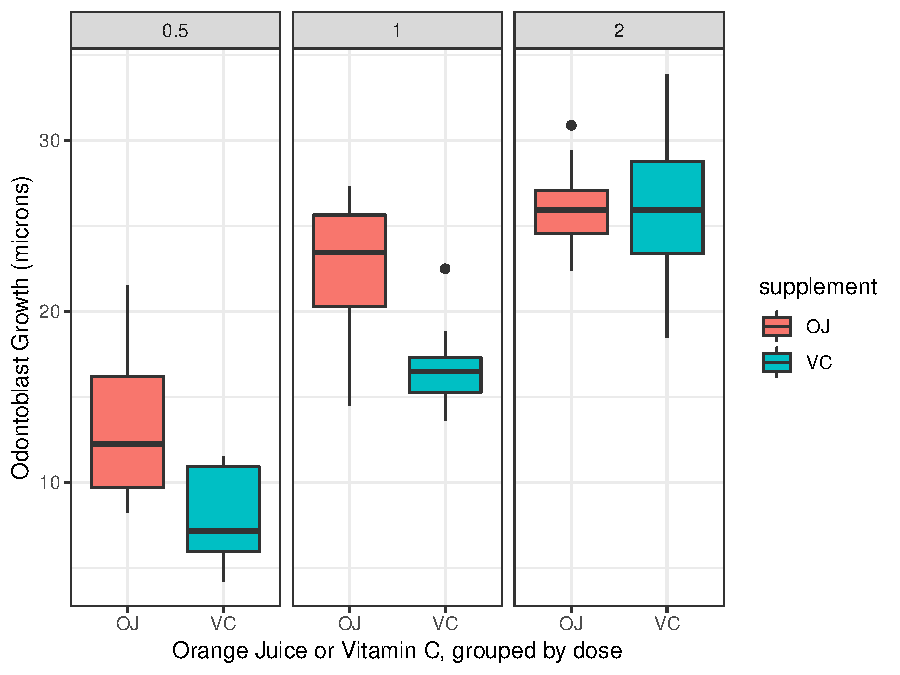
\includegraphics{UChicago-MScA-Capstone_files/figure-latex/boxplot-1.pdf}
\caption{\label{fig:boxplot}Avg. length by supplement and dose}
\end{figure}
Figure \ref{fig:boxplot} was created with the \texttt{ggplot2} package.
We can visually compare the average tooth growth by \texttt{supplement}
and \texttt{dose}.

\section*{Modeling results}\label{modeling-results}
\addcontentsline{toc}{section}{Modeling results}

First, use a \texttt{t.test()} to test \emph{if} dosage leads to growth
of incisor length. From the results below, it appears every test rejects
the null hypothesis.
\begin{Shaded}
\begin{Highlighting}[]
\NormalTok{test1 <-}\StringTok{ }\KeywordTok{t.test}\NormalTok{(length }\OperatorTok{~}\StringTok{ }\NormalTok{dose, ToothGrowth, dose }\OperatorTok\StringTok{ }\KeywordTok{c}\NormalTok{(}\FloatTok{0.5}\NormalTok{,}\DecValTok{1}\NormalTok{)) }
\NormalTok{test2 <-}\StringTok{ }\KeywordTok{t.test}\NormalTok{(length }\OperatorTok{~}\StringTok{ }\NormalTok{dose, ToothGrowth, dose }\OperatorTok\StringTok{ }\KeywordTok{c}\NormalTok{(}\FloatTok{0.5}\NormalTok{,}\DecValTok{2}\NormalTok{))}
\NormalTok{test3 <-}\StringTok{ }\KeywordTok{t.test}\NormalTok{(length }\OperatorTok{~}\StringTok{ }\NormalTok{dose, ToothGrowth, dose }\OperatorTok\StringTok{ }\KeywordTok{c}\NormalTok{(}\DecValTok{1}\NormalTok{,}\DecValTok{2}\NormalTok{)) }

\NormalTok{testAgg <-}\StringTok{ }\KeywordTok{data.frame}\NormalTok{(}\DataTypeTok{Name =} \KeywordTok{c}\NormalTok{(}\StringTok{"Test 0.5-1"}\NormalTok{, }\StringTok{"Test 0.5-2"}\NormalTok{, }\StringTok{"Test 1-2"}\NormalTok{),}
                  \DataTypeTok{Method =} \KeywordTok{c}\NormalTok{(test1}\OperatorTok{$}\NormalTok{method, test2}\OperatorTok{$}\NormalTok{method, test3}\OperatorTok{$}\NormalTok{method), }
               \DataTypeTok{Pvalue =} \KeywordTok{c}\NormalTok{(test1}\OperatorTok{$}\NormalTok{p.value, test2}\OperatorTok{$}\NormalTok{p.value, test3}\OperatorTok{$}\NormalTok{p.value), }
          \DataTypeTok{Tstat =} \KeywordTok{c}\NormalTok{(test1}\OperatorTok{$}\NormalTok{statistic, test2}\OperatorTok{$}\NormalTok{statistic, test3}\OperatorTok{$}\NormalTok{statistic))}

\KeywordTok{kable}\NormalTok{(testAgg, }\DataTypeTok{digit =} \DecValTok{7}\NormalTok{, }\DataTypeTok{align =} \StringTok{"r"}\NormalTok{, }\DataTypeTok{caption =} \StringTok{"t-test results"}\NormalTok{, }
      \DataTypeTok{format =} \StringTok{"latex"}\NormalTok{, }\DataTypeTok{longtable =} \OtherTok{TRUE}\NormalTok{)}
\end{Highlighting}
\end{Shaded}
\begin{longtable}{r|r|r|r}
\caption{\label{tab:t-test}t-test results}\\
\hline
Name & Method & Pvalue & Tstat\\
\hline
Test 0.5-1 & Welch Two Sample t-test & 1.00e-07 & -6.476648\\
\hline
Test 0.5-2 & Welch Two Sample t-test & 0.00e+00 & -11.799046\\
\hline
Test 1-2 & Welch Two Sample t-test & 1.91e-05 & -4.900484\\
\hline
\end{longtable}
Table \ref{tab:t-test}

\section*{Results of model performance and
validation}\label{results-of-model-performance-and-validation}
\addcontentsline{toc}{section}{Results of model performance and
validation}

Next, subset the \texttt{ToothGrowth} data into seperate data sets
defined by supplement dose of 0.5, 1, and 2 mg. This allow us to
controlling for dose increases of \emph{economic} significance.

Subset tooth data into a separate \texttt{data.frame} for each dosage
level. Then Execute the \texttt{t.test()} function for the dosage of 0.5
mg and display the results.
\begin{Shaded}
\begin{Highlighting}[]
\NormalTok{dose05 <-}\StringTok{ }\NormalTok{ToothGrowth[ToothGrowth}\OperatorTok{$}\NormalTok{dose }\OperatorTok{==}\StringTok{ }\FloatTok{0.5}\NormalTok{, ] }
\NormalTok{ dose1 <-}\StringTok{ }\NormalTok{ToothGrowth[ToothGrowth}\OperatorTok{$}\NormalTok{dose }\OperatorTok{==}\StringTok{ }\DecValTok{1}\NormalTok{, ]}
\NormalTok{ dose2 <-}\StringTok{ }\NormalTok{ToothGrowth[ToothGrowth}\OperatorTok{$}\NormalTok{dose }\OperatorTok{==}\StringTok{ }\DecValTok{2}\NormalTok{, ]}

\NormalTok{ test4 <-}\StringTok{ }\KeywordTok{t.test}\NormalTok{(length }\OperatorTok{~}\StringTok{ }\NormalTok{supplement, }\DataTypeTok{data =}\NormalTok{ dose05)}
\NormalTok{ test5 <-}\StringTok{ }\KeywordTok{t.test}\NormalTok{(length }\OperatorTok{~}\StringTok{ }\NormalTok{supplement, }\DataTypeTok{data =}\NormalTok{ dose1)}
\NormalTok{ test6 <-}\StringTok{ }\KeywordTok{t.test}\NormalTok{(length }\OperatorTok{~}\StringTok{ }\NormalTok{supplement, }\DataTypeTok{data =}\NormalTok{ dose2)}
\end{Highlighting}
\end{Shaded}
Place the results of the analysis directly into your content with
\textbf{\emph{inline code}} functions:

With a very low p-value of 0.0064 and a corresponding t-statistic of
3.1697, it appears that at low doses, \emph{Orange Juice} is the
preferable delivery mechanism to \emph{Vitamin C} for Ascorbic Acid
delivery.

The p-value and t-statistic above have been directly extracted from the
model object and printed inline. using the `r foo' syntax with quotes(')
replaced by back-ticks (`).

\chapter*{Conclusion}\label{conclusion}
\addcontentsline{toc}{chapter}{Conclusion}

This section includes a concise summary of the findings. Your summary
might be organized by the research objectives or hypotheses. Make sure
you address the extent to which research objectives are achieved, and if
they are not achieved, explain why. Make sure to interpret your findings
in a way that acknowledges the limitations of the research. That is, do
not extrapolate the insights derived from your research to situations
you have not examined.

\emph{While increasing dosage leads to larger incisor length, the choice
of delivery mechanism between Orange Juice and Vitamin C does not seem
to make a difference. However, at very low levels, Orange Juice appears
more effective, displaying higher average growth.}

\chapter*{Recommendations}\label{recommendations}
\addcontentsline{toc}{chapter}{Recommendations}

Includes guidelines as to ways in which your results should or could be
used in practice. You may discuss other uses of your results, if there
are any. The ways to extend your analysis and the benefits of doing so
might be included in this section as well.

\appendix

\chapter{The First Appendix}\label{the-first-appendix}

This first appendix includes all of the R chunks of code that were
hidden throughout the document (using the \texttt{include\ =\ FALSE}
chunk tag) to help with readibility and/or setup.

\textbf{In section} \ref{pressure-plot}:

\textbf{In section \ref{ref-labels}:}
\begin{Shaded}
\begin{Highlighting}[]
\KeywordTok{data}\NormalTok{(ToothGrowth)}
\KeywordTok{colnames}\NormalTok{(ToothGrowth) <-}\StringTok{ }\KeywordTok{c}\NormalTok{(}\StringTok{"length"}\NormalTok{, }\StringTok{"supplement"}\NormalTok{, }\StringTok{"dose"}\NormalTok{)}
\NormalTok{ToothGrowth}\OperatorTok{$}\NormalTok{dose <-}\StringTok{ }\KeywordTok{as.factor}\NormalTok{(ToothGrowth}\OperatorTok{$}\NormalTok{dose)}

\NormalTok{groupedTooth <-}\StringTok{ }\KeywordTok{aggregate}\NormalTok{(ToothGrowth, }\DataTypeTok{by=}\NormalTok{ToothGrowth[,}\DecValTok{2}\OperatorTok{:}\DecValTok{3}\NormalTok{], }\DataTypeTok{FUN=}\NormalTok{mean)[,}\DecValTok{1}\OperatorTok{:}\DecValTok{3}\NormalTok{]}

\KeywordTok{library}\NormalTok{(ggplot2)}
 \KeywordTok{ggplot}\NormalTok{(ToothGrowth, }\KeywordTok{aes}\NormalTok{(}\DataTypeTok{x =}\NormalTok{ supplement, }\DataTypeTok{y =}\NormalTok{ length)) }\OperatorTok{+}\StringTok{ }
\StringTok{                     }\KeywordTok{geom_boxplot}\NormalTok{(}\KeywordTok{aes}\NormalTok{(}\DataTypeTok{fill=}\NormalTok{supplement)) }\OperatorTok{+}\StringTok{ }
\StringTok{                     }\KeywordTok{facet_wrap}\NormalTok{(}\OperatorTok{~}\NormalTok{dose) }\OperatorTok{+}\StringTok{ }
\StringTok{                     }\KeywordTok{guides}\NormalTok{(}\DataTypeTok{colour =} \KeywordTok{guide_legend}\NormalTok{(}\StringTok{"Color = Supplement"}\NormalTok{)) }\OperatorTok{+}\StringTok{ }
\StringTok{                     }\KeywordTok{labs}\NormalTok{(}\DataTypeTok{x=}\StringTok{"Orange Juice or Vitamin C, grouped by dose"}\NormalTok{, }
                          \DataTypeTok{y=}\StringTok{"Odontoblast Growth (microns)"}\NormalTok{)  }\OperatorTok{+}
\StringTok{                     }\KeywordTok{theme_bw}\NormalTok{()}
\end{Highlighting}
\end{Shaded}
\chapter{A Second Appendix, for
example}\label{a-second-appendix-for-example}

\backmatter

\chapter*{References}\label{references}
\addcontentsline{toc}{chapter}{References}

\markboth{References}{References}

\noindent

\setlength{\parindent}{-0.20in} \setlength{\leftskip}{0.20in}
\setlength{\parskip}{8pt}

There are a variety of tools available for creating a bibliography
database (stored with the .bib extension). In addition to BibTeX
suggested below, you may want to consider using the free and easy-to-use
tool called \href{https://www.zotero.org/}{Zotero}.

\emph{R Markdown} uses \emph{pandoc} (\url{http://pandoc.org/}) to build
its bibliographies. To cite references in your thesis (after creating
your bibliography database), place the reference name inside square
brackets and precede it by the ``at'' symbol. For example, here's a
reference to a book about worrying: (Molina \& Borkovec, 1994). This
\texttt{Molina1994} entry appears in a file called \texttt{thesis.bib}
in the \texttt{bib} folder. This bibliography database file was created
by a program called BibTeX. You can call this file something else if you
like (look at the YAML header in the main .Rmd file) and, by default, is
to placed in the \texttt{bib} folder.

\textbf{Additional Tips}
\begin{itemize}
\tightlist
\item
  The sooner you start compiling your bibliography for something as
  large as a capstone, the better. Typing in source after source is
  mind-numbing enough; do you really want to do it for hours on end at
  the last minute?
\item
  The cite key (a citation's label) needs to be unique from the other
  entries.
\item
  When you have more than one author or editor, you need to separate
  each author's name by the word ``and'' e.g.
  \texttt{Author\ =\ \{Noble,\ Sam\ and\ Youngberg,\ Jessica\},}
\end{itemize}
\textbf{Example output generated from bib file}

\hypertarget{refs}{}
\hypertarget{ref-angel2000}{}
Angel, E. (2000). \emph{Interactive computer graphics : A top-down
approach with opengl}. Boston, MA: Addison Wesley Longman.

\hypertarget{ref-angel2001}{}
Angel, E. (2001a). \emph{Batch-file computer graphics : A bottom-up
approach with quicktime}. Boston, MA: Wesley Addison Longman.

\hypertarget{ref-angel2002a}{}
Angel, E. (2001b). \emph{Test second book by angel}. Boston, MA: Wesley
Addison Longman.

\hypertarget{ref-Molina1994}{}
Molina, S. T., \& Borkovec, T. D. (1994). The Penn State worry
questionnaire: Psychometric properties and associated characteristics.
In G. C. L. Davey \& F. Tallis (Eds.), \emph{Worrying: Perspectives on
theory, assessment and treatment} (pp. 265--283). New York: Wiley.


% Index?

\end{document}
